% 图 84.2 —— 由 `checks/emit_hand.py` 自动拼出（probe 精测 + prims2 图元分解）
%%
% ⚠ 这是**稿子不是成品**：跑 `checks/checkhand.py 84.2` 看指标 + 看叠合图。
%%
%% ⚠ 待核：
%   · 本图 probe 报出阴影族 1 个 —— **本脚本不生成阴影**（要照原书手写）；prims2 的 strokes 里可能含阴影线，核对时留意别画重
%   · 可疑字形 1 项（空心圈 ⊙ 常被认成字母 o）—— 见文件末
%%
\documentclass[12pt]{standalone}
\usepackage{fontspec}
\setsansfont{Arial}
\newfontfamily\mfallback{DejaVu Sans}
\usepackage{tikz}
\begin{document}
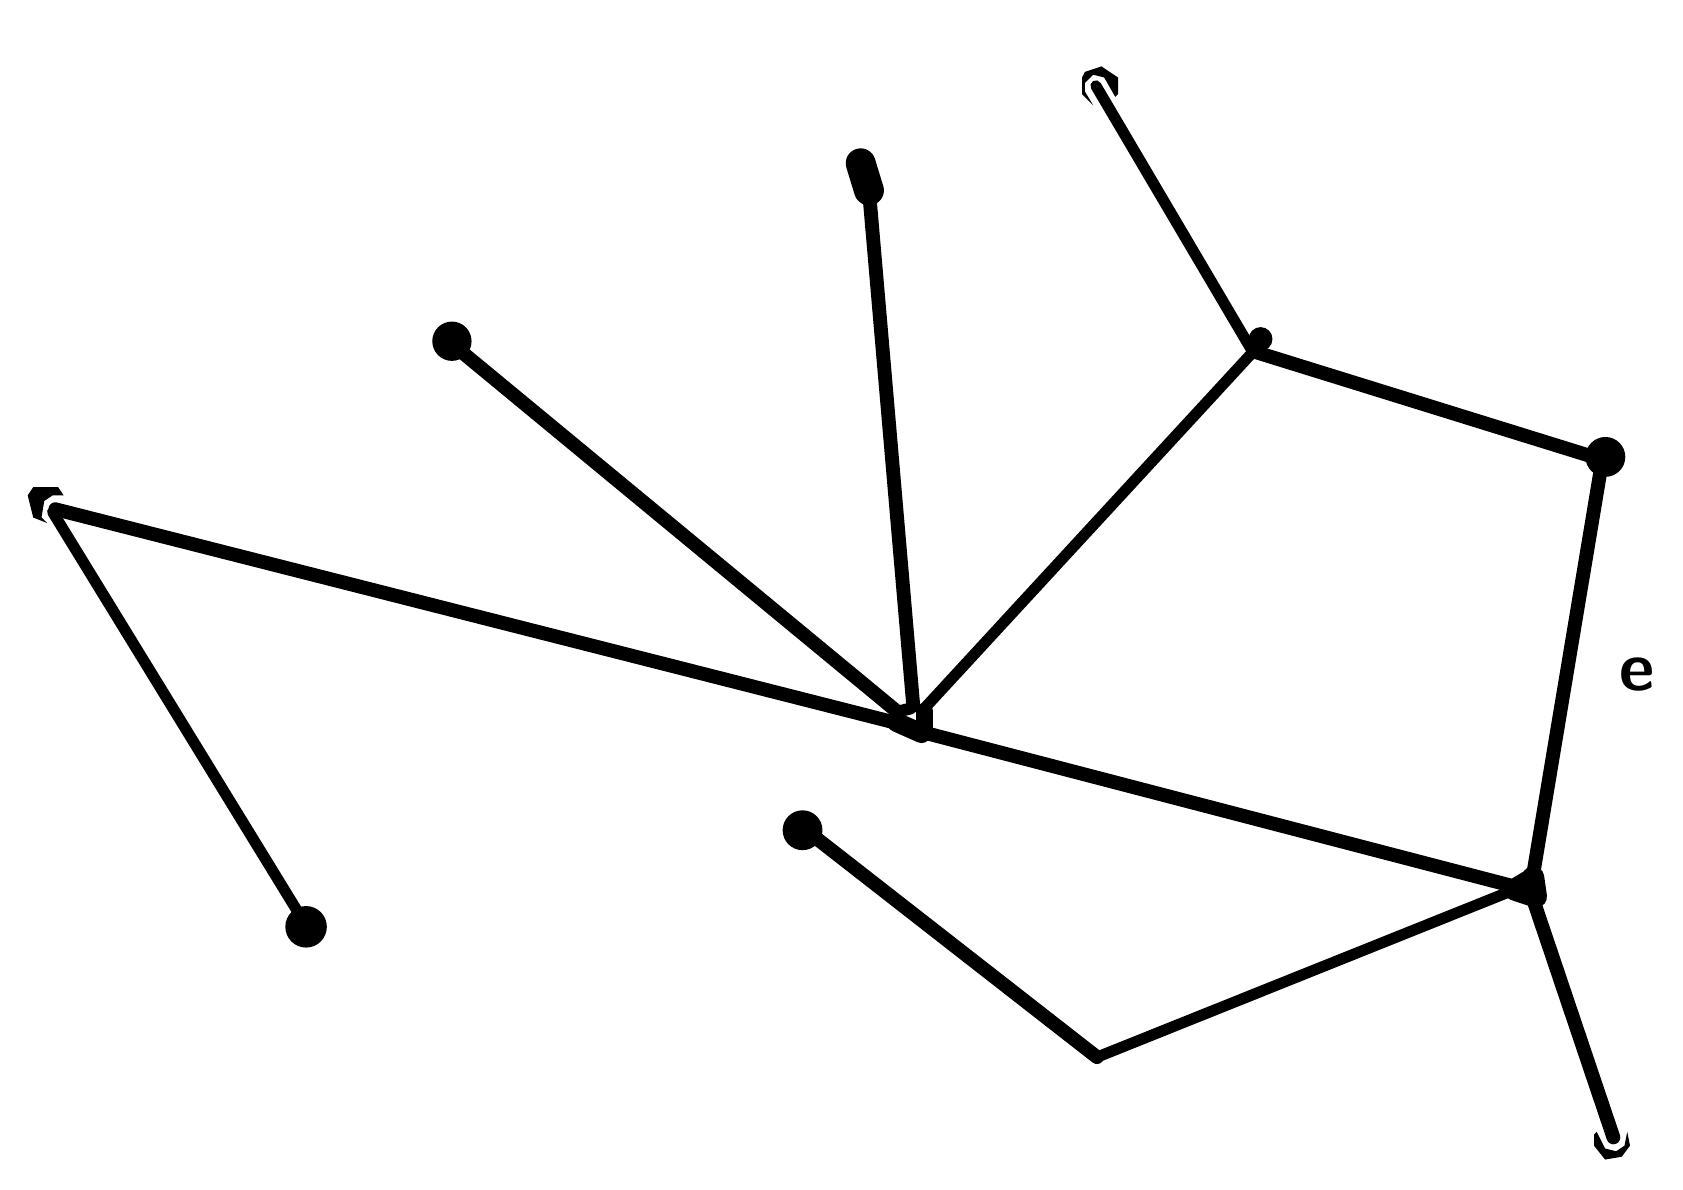
\begin{tikzpicture}[x=1pt, y=-1pt, line width=6.7pt, line cap=round, line join=round]

  %% ════ 填充区（prims2 的 fills）════
  \fill (388.0,14.0) -- (382.0,16.0) -- (381.0,18.0) -- (381.0,24.0) -- (385.0,28.0) -- (382.0,23.0) -- (382.0,20.0) -- (385.0,17.0) -- (389.0,18.0) -- (393.0,25.0) -- (394.0,24.0) -- (394.0,18.0) -- cycle;
  \fill (2.0,166.0) -- (0.0,169.0) -- (2.0,177.0) -- (7.0,179.0) -- (5.0,177.0) -- (6.0,171.0) -- (9.0,169.0) -- (13.0,169.0) -- (11.0,166.0) -- cycle;
  \fill (566.0,400.0) -- (566.0,404.0) -- (570.0,409.0) -- (576.0,408.0) -- (579.0,404.0) -- (578.0,399.0) -- (577.0,404.0) -- (574.0,406.0) -- (570.0,405.0) -- (567.0,399.0) -- cycle;

  %% ════ 直线段（prims2 的 strokes）════
  \draw[line width=6.7pt] (537.0,312.0) -- (543.0,314.0);
  \draw[line width=6.0pt] (324.0,254.0) -- (324.0,247.0);
  \draw[line width=7.0pt] (323.0,255.0) -- (314.0,251.0);
  \draw[line width=4.0pt] (442.0,116.0) -- (386.0,21.0);
  \draw[line width=5.0pt] (536.0,310.0) -- (325.0,255.0);
  \draw[line width=5.0pt] (313.0,251.0) -- (10.0,174.0);
  \draw[line width=4.0pt] (442.0,118.0) -- (324.0,246.0);
  \draw[line width=5.0pt] (544.0,315.0) -- (573.0,401.0);
  \draw[line width=4.3pt] (315.0,247.0) -- (319.0,246.0);
  \draw[line width=5.0pt] (544.0,306.0) -- (569.0,156.1);
  \draw[line width=5.0pt] (569.0,156.1) -- (443.0,117.0);
  \draw[line width=6.1pt] (543.0,307.0) -- (538.0,310.0);
  \draw[line width=4.0pt] (536.0,312.0) -- (386.4,372.0);
  \draw[line width=5.0pt] (386.4,372.0) -- (280.0,289.0);
  \draw[line width=4.0pt] (9.0,175.0) -- (101.0,325.0);
  \draw[line width=8.0pt] (545.0,314.0) -- (544.0,307.0);
  \draw[line width=5.0pt] (320.0,245.0) -- (304.0,58.8);
  \draw[line width=10.8pt] (304.0,58.8) -- (301.0,49.0);
  \draw[line width=5.0pt] (314.0,247.0) -- (153.0,114.0);

  %% ════ 实心点 ════
  \fill (153.3,113.3) circle (7.1);
  \fill (445.5,112.5) circle (4.3);
  \fill (570.1,155.1) circle (7.2);
  \fill (280.0,290.0) circle (7.2);
  \fill (100.6,324.9) circle (7.5);

  %% ════ 标签（probe 直接给的 \node 行）════
  %% ⚠ 全部补了 fill=white：文字在最上层，否则与曲线交叉干扰
     \node[anchor=center,inner sep=0pt,fill=white,font=\fontsize{35.2}{44.0}\selectfont] at (581.6,233.8) {\textsf{\textbf{\textit{e}}}};   % box(571,222,17,20)

  % 钉死画布：否则超出的图元/控制点会把页面撑大，1:1 回比就失准
  \pgfresetboundingbox
  \path[use as bounding box] (0,0) rectangle (588,410);
\end{tikzpicture}
\end{document}

% ⚠ 待核清单（probe 拿不准，人眼过一遍）：
%   · 未识别/跳过：⑤ 跳过/未识别的字形
